\section{Results}


\subsection{Optic Microscopy}

\begin{figure}[h!]
	\begin{center}
		\begin{tabular}{ccc}
			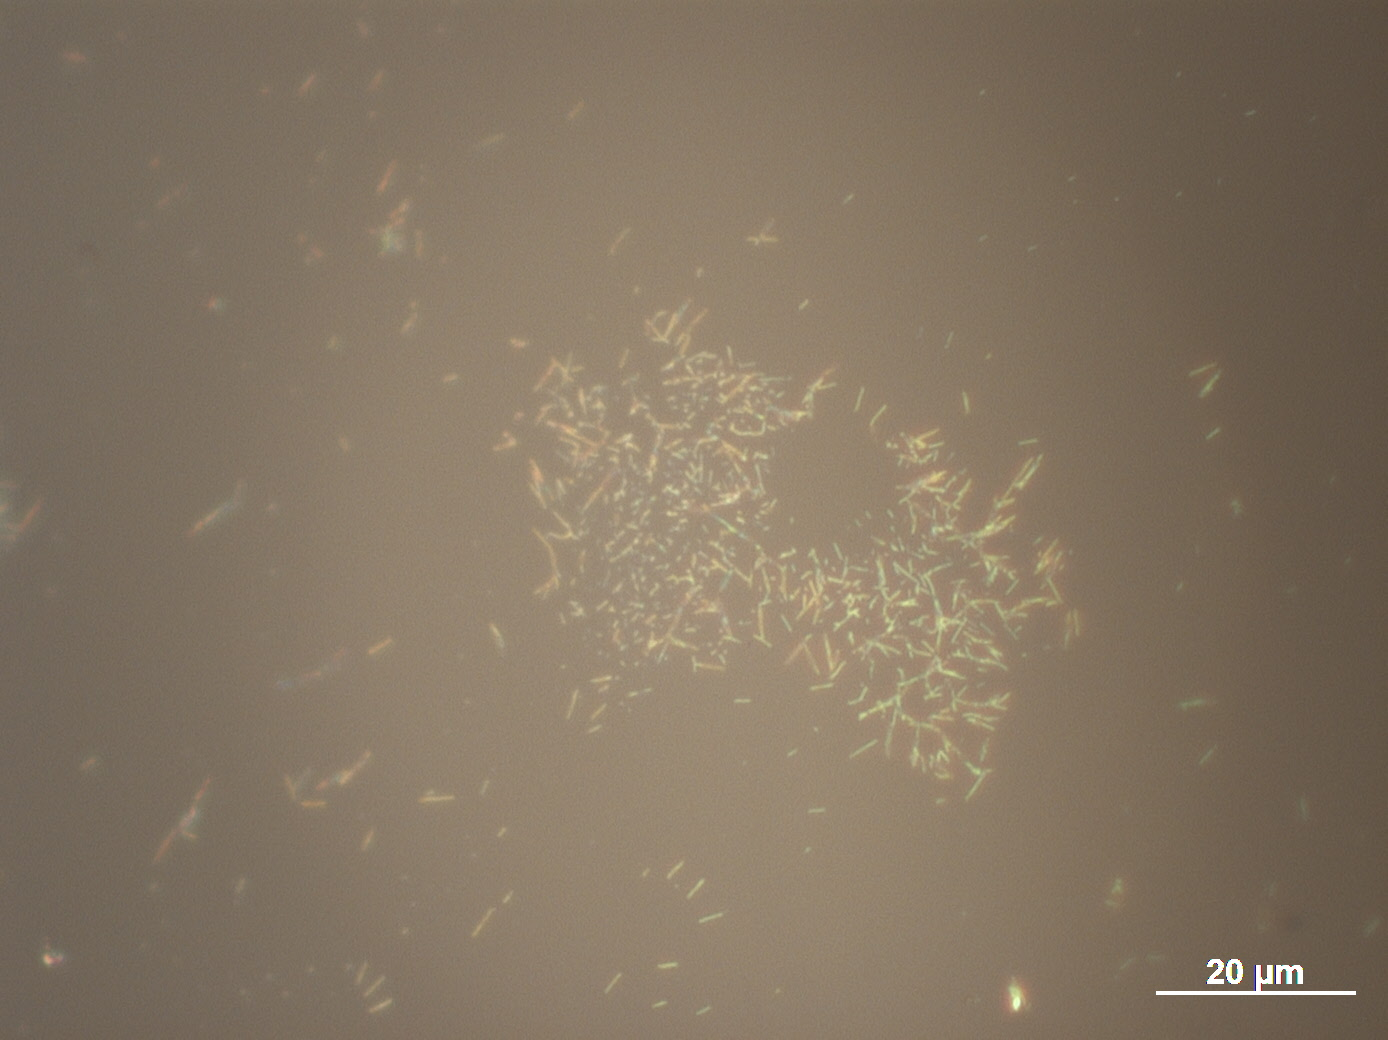
\includegraphics[height=4cm]{optic} &   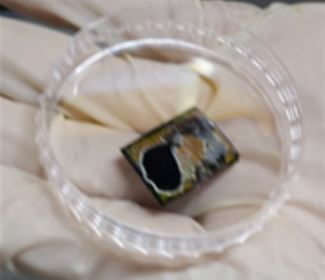
\includegraphics[height=4cm]{crystal}&
			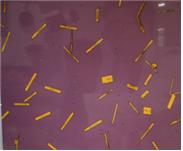
\includegraphics[height=4cm]{crystal_made}
		\end{tabular}
		\caption{(a) The picture shows the silicon wafer with no crystals. After the crystal successfully grew, it could be seen by the eyes,(b) and (c) by optic microscopy.}	
		\label{fig:FIR221}
	\end{center}
\end{figure}
\subsection{X-Ray Diffraction}
\begin{figure}[h!]
	\begin{center}
		\begin{tabular}{c}
			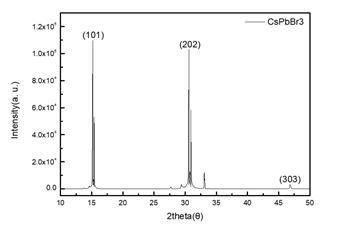
\includegraphics[width=10cm]{XRD}
		\end{tabular}
		\caption{The angle of incidence was varied 10 to 70 degrees. The graph was drawn with Origin 8.0}	
		\label{fig:FIR221}
	\end{center}
\end{figure}
$\rm{CsPbBr_3}$의 XRD peak는 2θ = 14.919, 30.099, 47.957도에서 발견되는 기존의 데이터와 일치하기 때문에 XRD 분석을 통해 $\rm{CsPbBr_3}$ 결정이 만들어졌다는 것을 알 수 있다 \cite{Jain2013}.

\subsection{TRPL spectroscopy}
\begin{figure}[h]
	\begin{center}
		\begin{tabular}{c}
			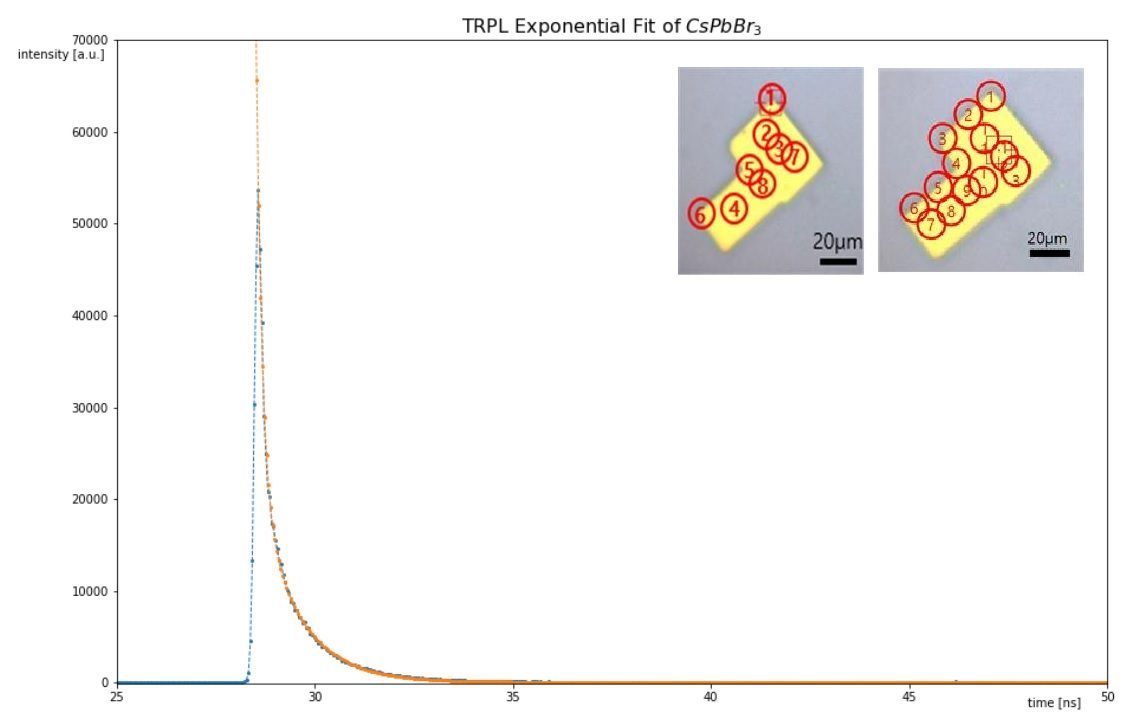
\includegraphics[width=14cm]{TRPL_graph}
		\end{tabular}
		\caption{TRPL graph was fitted with sum of exponential functions.x axis is time(ns) y axis is the intensity of signal(a.u.). Two pictures at the right top shows the point where the TRPL datas were collected. Left picture corresponds to ND0 filter,and the right picture corresponds to ND1 filter. }	
		\label{fig:FIR221}
	\end{center}
\end{figure}
TRPL 그래프는 위의 그림과 같이 파란색의 그래프이다. t=28 ns부근에서 최댓값을 확인 할 수 있었고, 그 시간 이후의 데이터를 시간에 따른 지수 함수(exponential function)들의 합으로 fitting 할 수 있는데, 그 식은 $\sum_{i}^{} {e}^{-t/{\tau}_{i}}$ 로 표현된다. $\rm{CsPbBr_3}$는 exciton과 biexciton의 recombination으로 나뉘기 때문에 두 개의 exponential function의 합으로 표현하였다. 

그래프의 피팅을 위해 파이썬을 활용하였다. TRPL 데이터를 순서쌍으로 바꿔서 그래프를 그린 후, 파이썬에 내재된 함수인 curve fit을 이용하여 최소제곱법으로 가장 비슷한 함수를 찾아낸다.
\begin{figure}[t]
	\begin{center}
		\begin{tabular}{cc}
			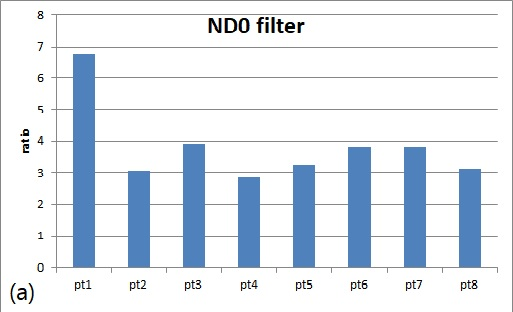
\includegraphics[height=4cm]{ND0} &
			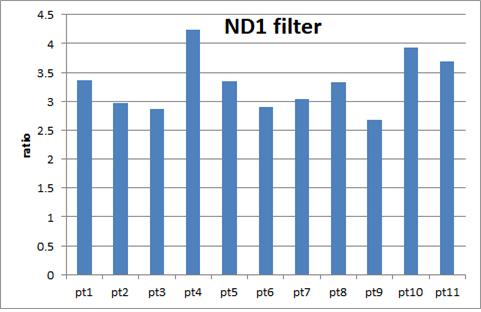
\includegraphics[height=4cm]{ND1}
		\end{tabular}
		\caption{The histogram shows the ratio between exciton recombination rate and biexcitonrate, differed by the point of laser. (a) is when ND0 filter is used, and (b) is when ND1 filter is used. The standard deviation of ratio is 0.432 and 0.483, respectively. }	
		\label{fig:FIR221}
	\end{center}
\end{figure}

\begin{figure}[t]
	\begin{center}
		\begin{tabular}{cc}
		\begin{tikzpicture}
		\begin{axis} [
		width=0.50\textwidth,%
		height = 6cm,%
		ybar,%
		title={ND0 filter},%
		xtick = data,%
		symbolic x coords={pt1, pt2, pt3, pt4, pt5, pt6, pt7, pt8},%
		ylabel= {ratio},%
		ymin=0,ystep=0.5,ymax=10.0,%
		scaled y ticks = false,%
		ymajorgrids = true,
		legend style={at={(0.02,10)}},legend pos=north west]%
		\addplot table [x=pt, y=data] {./pt_data/ratio_nd0.csv}; %\addlegendentry {2003 LAC}%
		\end{axis}
		\node at (-0.2, 5.0) {(a)};
		\end{tikzpicture}
		&
		\begin{tikzpicture}
		\begin{axis} [
		width=0.50\textwidth,%
		height = 6cm,%
		ybar,%
		title={ND1 filter},%
		xtick = data,%
		symbolic x coords={pt1, pt2, pt3, pt4, pt5, pt6, pt7, pt8, pt9, pt10, pt11, pt12, pt13},%
		ylabel= {ratio},%
		ymin=0,ystep=0.5,ymax=10.0,%
		scaled y ticks = false,%
		ymajorgrids = true,
		legend style={at={(0.02,10)}},legend pos=north west]%
		\addplot table [x=pt, y=data] {./pt_data/ratio_nd1.csv}; %\addlegendentry {2003 LAC}%
		\end{axis}
		\node at (-0.2, 5.0) {(b)};
		\end{tikzpicture}	
		\end{tabular}		
	\caption{The histogram shows the ratio between exciton recombination rate and biexcitonrate, differed by the point of laser. (a) is when ND0 filter is used, and (b) is when ND1 filter is used. The standard deviation of ratio is 0.432 and 0.483, respectively. }	
		\label{fig:FIR221-1}
	\end{center}
\end{figure}

 만들어진 결정이 $\rm{CsPbBr_3}$ 임을 확인하기 위해서 exciton과 biexciton의 recombination rate에 대한 비율을 계산하였다. 
ND0 필터를 사용했을 때 두 recombination rate 사이의 비율에 대한 평균값은 3.43 이었고 ND1필터를 사용 했을 때는 3.30이었다.
\clearpage
\begin{figure}[h]
	\begin{center}
		\begin{tabular}{cc}
			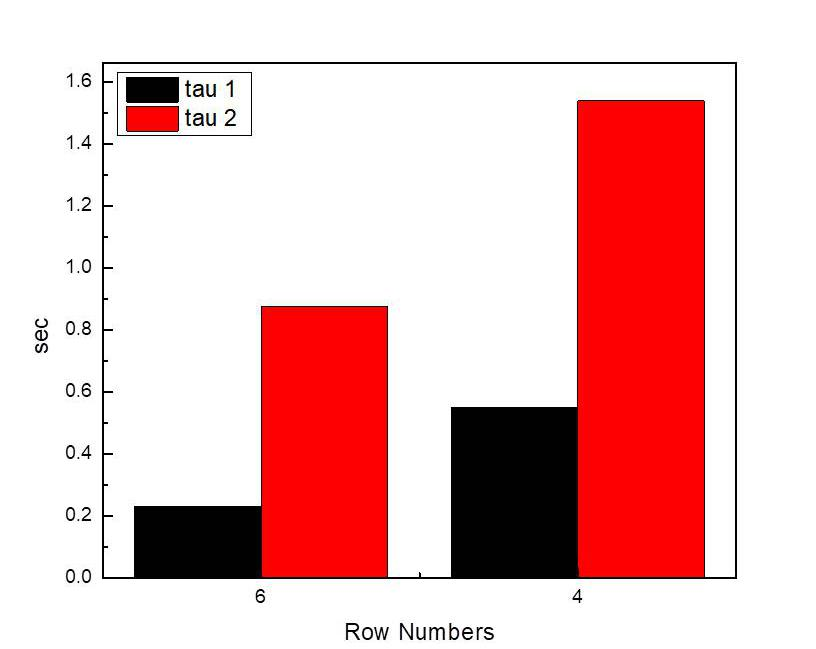
\includegraphics[width=7cm]{ND0TRPL1} &
			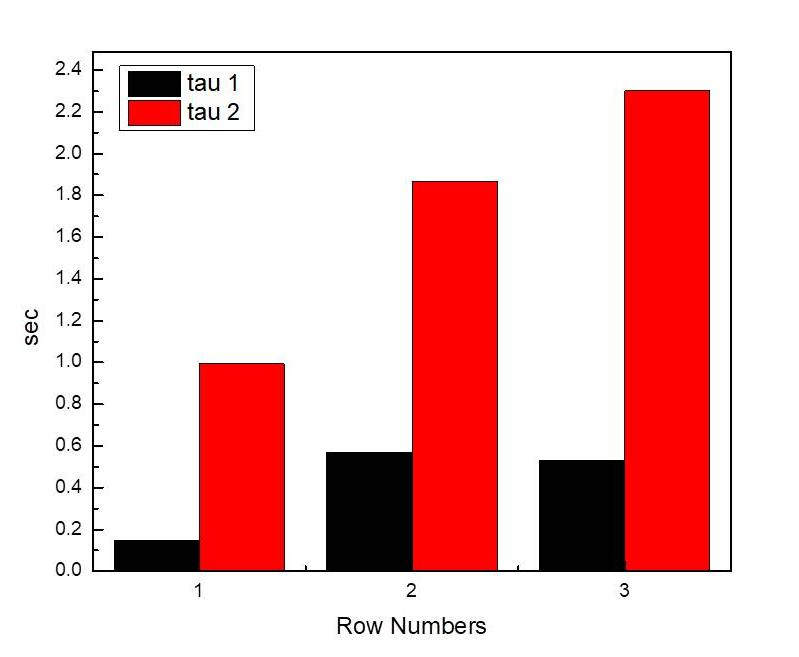
\includegraphics[width=7cm]{ND0TRPL2}\\
			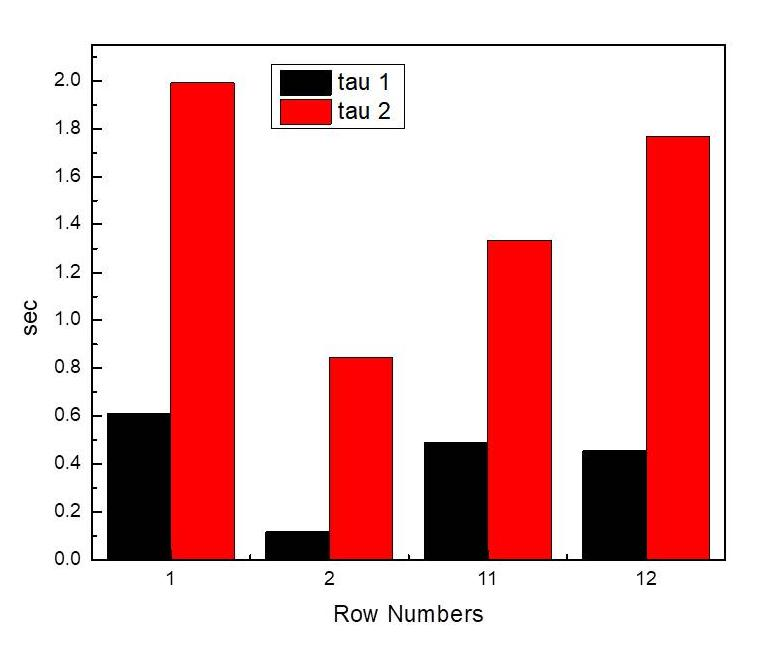
\includegraphics[width=7cm]{ND1TRPL1} &
			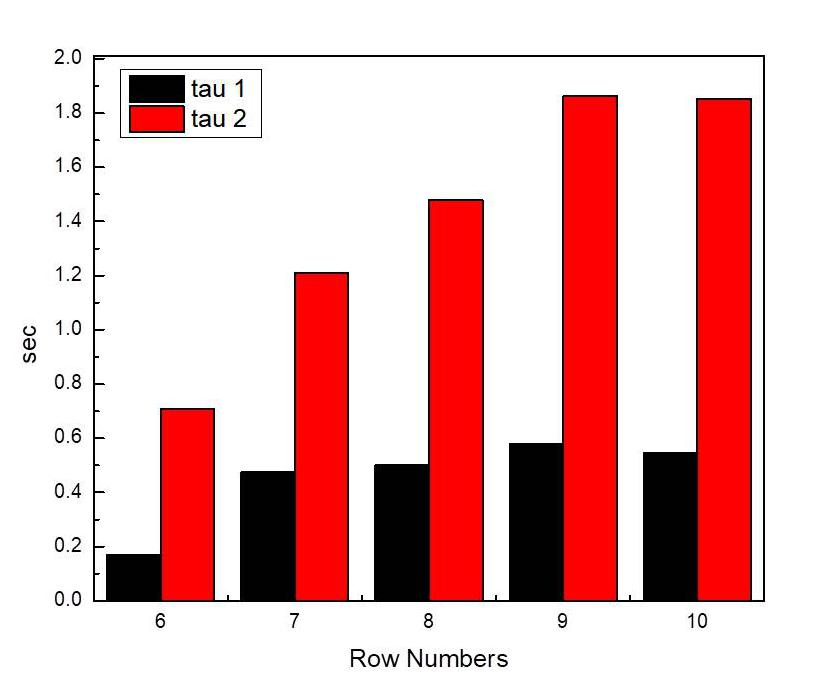
\includegraphics[width=7cm]{ND1TRPL2}
		\end{tabular}
		\caption{Both exciton / biexciton recombination rate increased when the laser point headed to the center of the crystal. The unit of y-axis is ns.}	
		\label{fig:FIR221}
	\end{center}
\end{figure}
Figure 7은 exciton / biexciton recombination rate의 비율이 아닌, 값 자체를 히스토그램으로 나타낸 것으로, 두 값 모두가 결정의 중심쪽으로 갈수록 증가하고 있음을 관찰할 수 있다. 